%%%%%%%%%%%%%%%%%%%%%%%%%%%%%%%%%%%%%%%%%%%%%%%%%%%%%%%%%%%%%%%%%%%%%% LE RADICI
%%%%%%%%%%%%%%%%%%%%%%%%%%%%%%%%%%%%%%%%%%%%%%%%%%%%%%%%%%%%%%%%%%%%%%%%%%%%%%%%
\section{Le Radici}

L'“International Exposition of Electricity", tenutasi nel 1881, ha mostrato cose come l'illuminazione elettrica con Edison e altri che presentano le loro lampadine a incandescenza.

Uno dei reperti era un "telefono stereo". Nel 1881 Alexander Graham Bell aveva un modello funzionante del suo telefono, ma era il francese Clément Ader la cui invenzione fu esposta [2]. Forse la ragione è stata la decisione del governo britannico di non sprecare denaro pubblico sponsorizzando l'evento. Ogni sera veniva suonata musica alla Grande Opera e la gente poteva ascoltare per alcuni minuti al telefono a circa due chilometri di distanza al Palais de Industrie, dove si teneva l'esposizione. Una serie di dieci microfoni al carbonio è stata posizionata lungo la larghezza del palco. Ciascuno di questi era collegato a otto stazioni di ascolto all'estremità opposta. Si potrebbe pensare che, dato che il telefono era ancora agli inizi, per i membri del pubblico semplicemente ascoltare la performance sarebbe stato sufficiente, ma Ader ha aggiunto l'esperienza di "stereo". Ogni persona che ascoltava aveva due auricolari, uno per ciascun orecchio. Ogni auricolare ha presentato la performance da una posizione separata sul palco (ad es. Microfoni 1 e 6, 2 e 7, e così via) consentendo così all'ascoltatore di valutare la posizione laterale dell'esecutore. Fortunatamente, l'esperimento ebbe successo e nacque "stereo". Diversi anni dopo l'Expo di Parigi del 1881, l'invenzione fu usata commercialmente in Francia e in Inghilterra. Il telefono e la rete richiesta furono sviluppati, così come la distribuzione di energia elettrica, ma il prossimo traguardo per lo stereo non sarebbe arrivato fino a 50 anni dopo.

%------------------------- APPROFONDIMENTO
\begin{tabular}{L{.969\textwidth}}%
\toprule
	\textbf{Alan Dower Blumlein}\\
\midrule
Nato il 29 giugno 1903 a Londra, Deceduto il 7 giugno 1942 a Herefordshire,
Inghilterra, fu ingegnere elettronico presso EMI, per la quale pubblicò brevetti
per le sue numerose invenzioni nel campo delle telecomunicazioni soprattutto in
relaizone alle tecnologie di registrazione, trasmissione e diffusione del suono.
Ottiene, nella sua breve carriera, 128 brevetti, motivo per cui è considerato
uno dei più importanti ingegneri e inventori del suo tempo. Morì durante la
seconda guerra mondiale all'età di 38 anni, durante un test militare segreto del
sistema radar H2S allora in fase di sviluppo, a bordo del bombardiere Halifax
su cui stava volando. Tra le numerose invenzioni legate al nome di Blumlein
quelle legate alla Stereofonia stravolsero completamente il mondo della
fruizione pubblica del suono. Le sue prime note sull'argomento risalgono al 25
settembre 1931 e il suo brevetto aveva il titolo “Miglioramenti ai, ed in
relazione ai, sistemi di trasmissione, registrazione e riproduzione del suono”.
La domanda di brevetto fu del 14 dicembre 1931 ed la concessione fu dell
14 giugno 1933, brevetto britannico numero 394.325.\\
\bottomrule
\end{tabular}
%------------------------- APPROFONDIMENTO

\clearpage

La percezione dei caratteri spazio-temporali dei suoni, in particolare della
loro direzione di provenienza e della loro relazione con lo spazio che
attraversano, definiscono i tratti essenziali della stereofonia, in relazione
all'udito, in virtù dell’audizione biauricolare (o binaurale). Come sottolineato
nell'enciclopedia Treccani, tra le varie definizioni di stereofonia \emph{il
termine è inoltre usato per indicare la parte dell’acustica fisiologica
che si occupa di tale fenomeno}. L'ascolto biauricolare del sistema uditivo
conferisce alla percezione umana il potere localizzatore, cioè la capacità,
dovuta al lavoro congiunto dei due sistemi auricolari separati ed al sistema
nervoso centrale, di determinare la direzione di provenienza di un suono. In tal
senso, esiste in acustica fisiologica la definizione di monofonia in qualità di
condizione anomala del sistema percettivo, caratterizzata dalla mancanza degli
elementi necessari a individuare i caratteri spaziali dei suoni stessi, come per
esempio quella ottenuta con un solo orecchio.

L'ultimo esercizio linguistico è legato alla definizione dell'aggettivo
\emph{stereofònico} e ci permette di aprire il termine alle tecniche ed alle
tecnologie che hanno reso possibile la trasmissione, la riproduzione,
e la diffusione della stereofonia. \emph{Stereofònico}, quindi, che si riferisce
alla stereofonia, alla percezione della stereofonia, alla descrizione delle
tecniche di registrazione e riproduzione in grado di operare stereofonia. Un
aggettivo che dovrebbe essere usato solo nella
descrizione di tecniche di registrazione e di diffusione sonora atte alla
riproduzione dei suoni in modo che l’ascoltatore abbia l’impressione di trovarsi
nello spazio sonoro originale, dai quali ne deriva una musica stereofonica ed
una discografia stereofonica in grado di grarantire l’ambiente sonoro originale,
solido e tridimensionale attraverso l’effetto stereofonico.

\begin{quotation}
An observer in the room is listening with two ears, so that echoes reach him
with the directional significance which he associates with the music performed
in such room. He therefore discount these echoes and psychologically focuses
his attention on the source of the sound. When the music is reproduced through
a single channel the echoes arrive from the same direction as the direct sound
so that confusion results. [\ldots] Human ability to determine the direction
from which sound arrives is due to binaural hearing, the brain being able to
detect differences between sound received by the two ears from the same source
and thus to determine angular directions from which various sounds
arrive\footnote{Un osservatore nella stanza sta ascoltando con due orecchie, in
modo che gli echi lo raggiungano con il significato direzionale che associa alla
musica eseguita in quella stanza. Pertanto, non tiene conto di questi echi e
focalizza psicologicamente la sua attenzione sulla fonte del suono. Quando la
musica viene riprodotta attraverso un singolo canale, gli echi arrivano dalla
stessa direzione del suono diretto, in modo da creare confusione. [...] La
capacità umana di determinare la direzione da cui proviene il suono è dovuta
all'udito binaurale, il cervello è in grado di rilevare le differenze tra il
suono ricevuto dalle due orecchie dalla stessa fonte e quindi di determinare le
direzioni angolari da cui provengono i vari suoni.}. [\cite{ab58}]
\end{quotation}

Con queste parole Blumlein nel 1931 descrive i fondamenti di almeno due grandi
argomenti: quali erano le conoscenze  dell'epoca su come percepiamo i suoni
acustici e come abbiamo riprodotto i suoni fino a quel momento.

La binauralità dell'ascolto umano è la prima affermazione di Blumlein:
“\emph{un osservatore nella stanza sta ascoltando con due orecchie}”. Come
questa condizione di ascolto si evolva nel tempo è la peculiarità della
stereofonia.

% Non è correlato al numero di fonti, nemmeno al numero di microfoni
% e altoparlanti necessari per riprodurre tale condizione. La tecnica e lo scopo
% della tecnica prescelta si concentreranno per risolvere più argomenti possibili
% per soddisfare tale condizione.

%%%%%%%%%%%%%%%%%%%%%%%%%%%%%%%%%%%%%%%%%%%%%%%%%%%%%%%%%%%%%%%%%%%%%%%%%%%%%%%%%%%%%%%%%%%%%%%%%% dalle esposizioni
Dovremmo indicare quindi qualitativamente una condizione di ascolto, dal latino
\emph{auscultare}, prestare attenzione a qualcosa in quanto oggetto o motivo di informazione, con specifiche caratteristiche di solidità spaziale, dimensionalità osservabili nella forma sonora riconoscibile, informativa.

\emph{Una voce in una piccola stanza riverberante è una condizione d'ascolto che
rispetti queste qualità?}

Prima di approfondire questioni di propagazione e percezione del suono, val la pena
dedicare un tempo alla letteratura specializzata.

\begin{quote}
When recording music considerable trouble is experienced with the unpleasant
effects produced by echoes wich in the normal way would not be noticed by anyone
listening in the room in which the performance is taking place. An observer in
the room is listening with two ears, so that echoes reach him with the directional
significance which he associates with the music performed in such room. He,
therefore, discounts these echoes and psychologically focuses his attention on
the source of the sound\footnote{Quando si registra musica acustica, si riscontrano
notevoli problemi a causa degli effetti indesiderati prodotti dalle riflessioni
acustiche dell'ambiente, che nell'ascolto normale non vengono notati dagli
ascoltatori nella stanza in cui si svolge l'esibizione. L'ascoltatore, nella stanza,
ascolta attraverso le due orecchie, le riflessioni lo raggiungano con il significato direzionale che associa alla musica eseguita in quella stanza.
Pertanto, elimina dal messaggio le informazioni delle riflessioni e focalizza
psicologicamente la sua attenzione sulla sorgente sonora.}.
\end{quote}

Richiesta di brevetto numero 394325 del 14 dicembre 1931, accettazione del 14
giugno 1933. Alan Dower Blumlein.

La risposta alla domanda \emph{Una voce in una piccola stanza riverberante è una
condizione d'ascolto che rispetti queste qualità?} è, in funzione di quanto
appena letto, chiaramente affermativa.

Anche con un solo oggetto sonoro, una sola voce, in una piccola stanza, siamo in
presenza di un fenomeno acustico stereofonico. Almeno così dice Blumlein, papà
della stereofonia, nel brevetto in cui ne rende i concetti fondamentali, solidi,
stabili nel tempo e nello spazio delle parole, nel brevetto tecnologico che stabilisce
il \emph{point break} dell'elettroacustica, per il resto dell'umanità.

\begin{figure}[h]
\begin{center}
  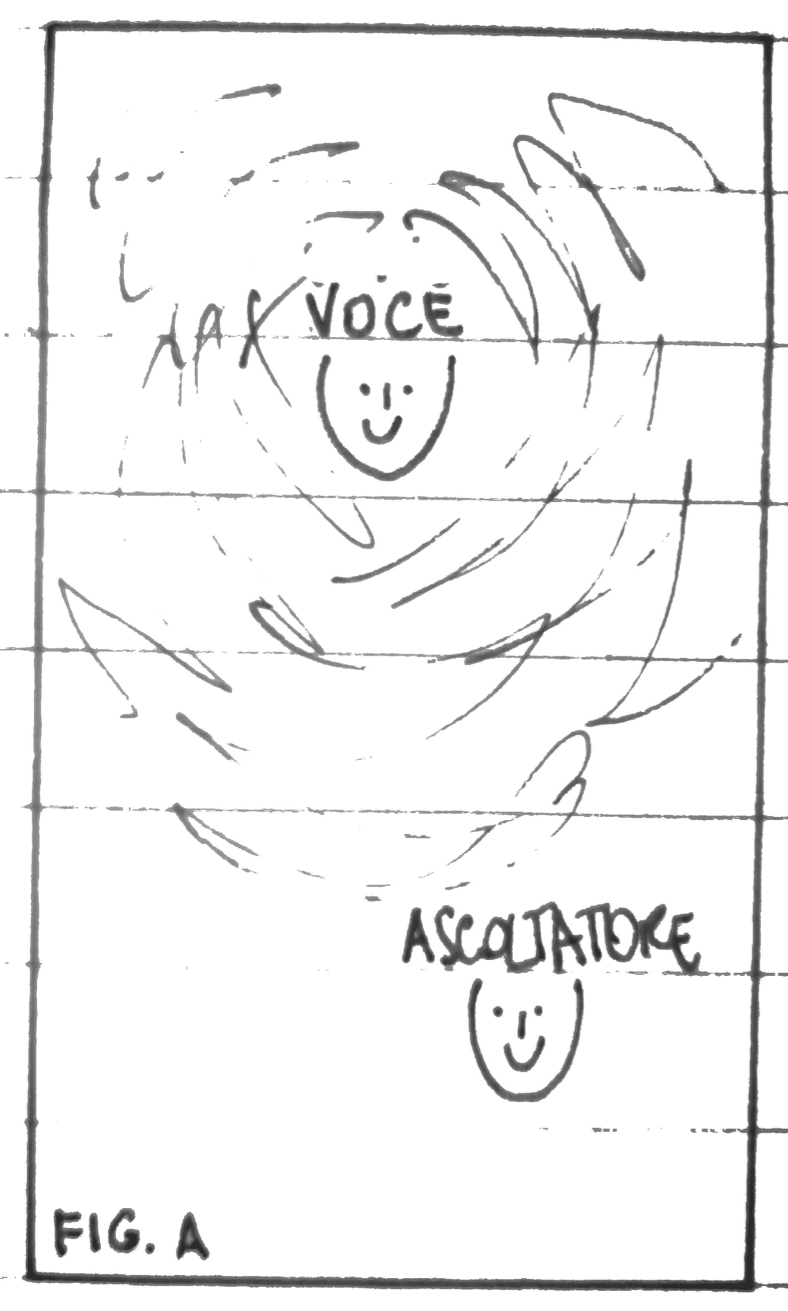
\includegraphics[width=.48\linewidth]{CAPITOLI/1000/IMG/figa.png}
%\caption{}
\label{ee:figa}
\end{center}
\end{figure}

Una voce nello spazio di una stanzetta si dirige, con una sua direzione, verso
un punto e contemporaneamente, con meno direzionalità, lateralemente, raggiunge
il resto della stanza. Questo meccanismo ha a che fare con la forma sonora di una
voce, prima ancora che con la forma architettonica della piccola stanza.

Dobbiamo immaginare la forma sonora come un'armatura attorno al nostro oggetto
sonoro, un'armatura fatta di fittissime molecole in vibrazione. Ogni suono ha una
sua veste plastica. Se vi dicessi ottavino e poi contrabbasso voi avreste già
collegato tutto ciò che vi serve per vederli, sentirli, ed ora, volendo, vestirli
della loro forma sonora. Ma cosa accade alla forma sonora di uno strumento in
presenza di tecninche estese applicate allo strumento? Una mano che inizia a produrre
suono li, nello stesso luogo dello strumento, a dove pochi minuti prima premeva
solo tasti (la mano  sinistra di UR) diventa esplosione di forma acustica e musicale.

Ecco questo è un po' il cuore di quello che vorrei fosse il mio dottorato di
ricerca che non avrò mai e un po' anche la manifestazionne di una piuttosto
triste verità: esclusi i percorsi individuali e rari percorsi di ricerca
non istituzionalizzata, la musica contemporanea ha esaurito la sua carica
contributiva al conoscimento, alla comprensione generalizzata.

Tornando alla forma, Questa si staglia nello spazio circostante e si espande e si muove
all'interno di questo spazio e ne viene modellata come una massa morbida all'interno
di un contenitore. Qui iniziano i fenomeni di riflessione e la forma si
cristallizza assumendo caratteristiche in funzione dello spazio e, quindi, del tempo.
L'ascoltatore che partecipa a questo evento vede una persona solida parlare nello
spazio di una stanza e sente la forma solida della voce provenire dalla sua bocca
e contemporaneamente, quindi subito dopo, dalla stanza sotto forma di riflessioni.
Sì! converremo infine, questa esperienza di ascolto rispetta queste qualità.

\begin{figure}[h]
\begin{center}
  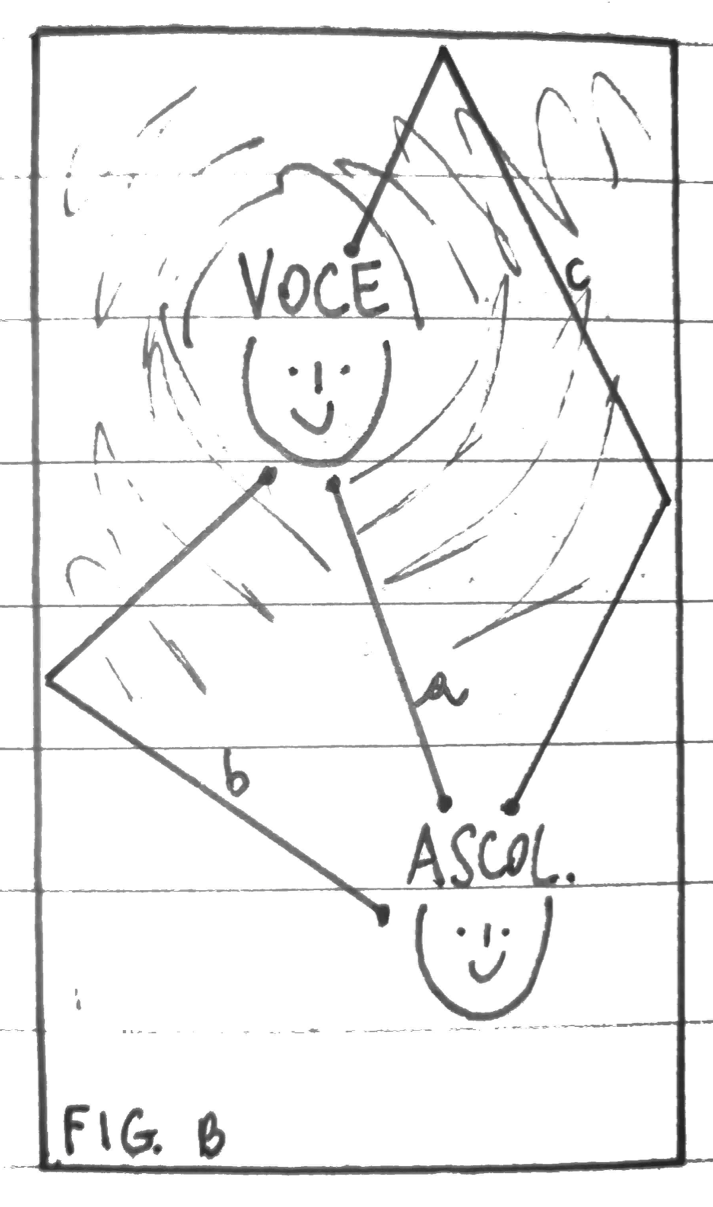
\includegraphics[width=.48\linewidth]{CAPITOLI/1000/IMG/figb.png}
%\caption{}
\label{ee:figb}
\end{center}
\end{figure}

Una voce che attraverso la sua forma acustica riempia uno spazio acustico è
un'esperienza d'ascolto stereofonica. Non è ancora giunto il momento di
interrompere la discussione dicendo: “ma come, non servono due diffusori?” Non
ancora, il problema è più complesso. È importante sottolineare che la stereofonia,
l'ascolto stereofonico, è una qualità dell'ascolto che si può osservare in
determinate circostanze e che richiede necessariamente il lavoro concertato delle
due orecchie. Un ascolto stereofonico è quindi possibile solo in coincidenza
con un ascolto \emph{binaurale}, ovvero effettuato con entrambe le orecchie.

Di nuovo una qualità che presuppone dei contenuti coerenti con delle
caratteristiche specifiche. Ora, nel mondo elettroacustico, del suono prodotto
o riprodotto elettricamente, dovremmo essere in grado di effettuare lo stesso
ragionamento sostituendo alla persona che parla un diffusore generico. Come per
l'essere umano, la voce è esempio di suono proprietario anche per il diffusore
si può scegliere un suono che lo caratterizzi elettroacusticamente, un suono
che lo rende particolare: il suono definito rumore rosa. Posizionato il diffusore
nella stessa stanza e con le stesse circostanze di ascolto precedenti, avremmo
una condizione di ascolto stereofonico? Ovviamente si. Un solo diffusore può
costituire una condizione d'ascolto stereofonica. In questo caso l'oggetto
acustico è un diffusore che esprime se stesso attraverso un suono non informativo.
Un rumore è caratterizzato da un'assenza di informazione, fatta esclusione del
fatto stesso che è rumore.

\begin{figure}[h]
\begin{center}
  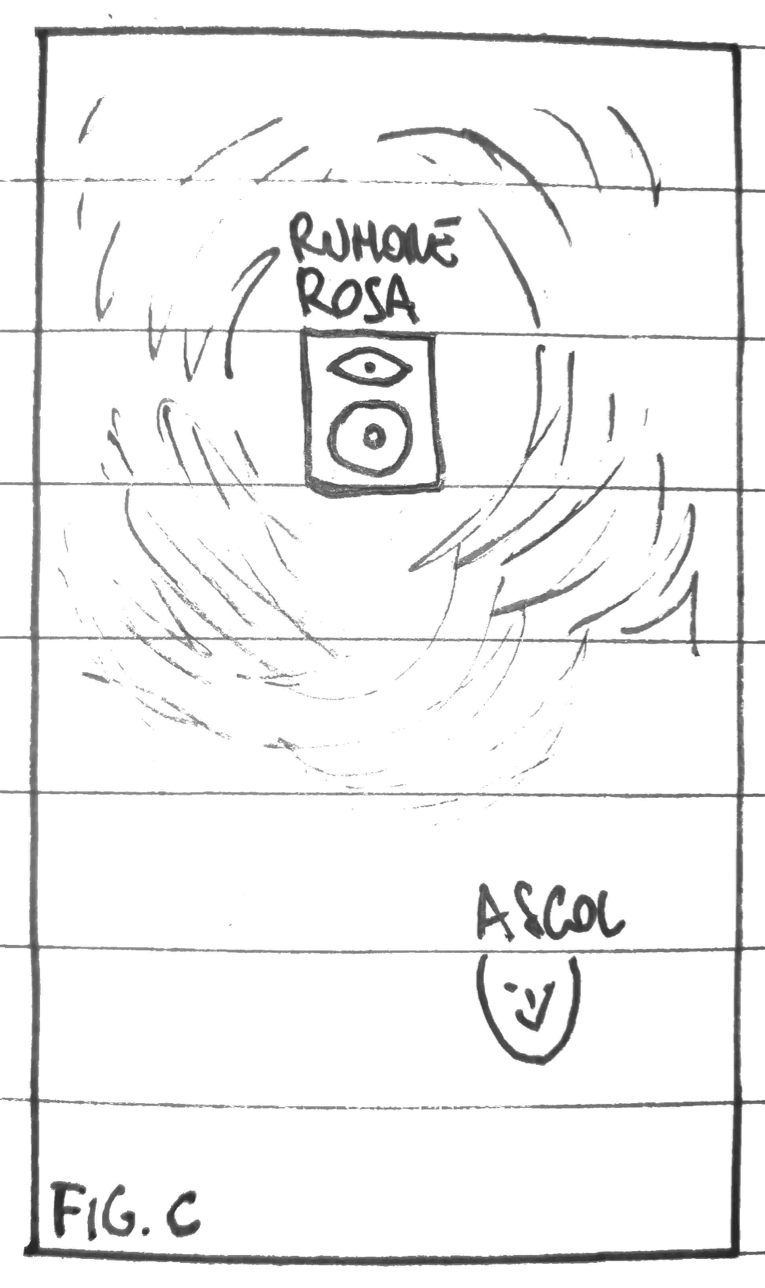
\includegraphics[width=.48\linewidth]{CAPITOLI/1000/IMG/figc.png}
%\caption{}
\label{ee:figc}
\end{center}
\end{figure}

che informazioni? be quelle che descrivono un suono come la percezione di altezza,
durata, intensità e timbro. Questa descirizione di stereofonia possibile anche
con un solo soggetto sonoro, voce o diffusore che sia, non è così comune e
condivisa. Ciò accade a causa del fatto che spesso si fa confusione tra stereofonia,
o stereofonica, come aggettivo applicato alla tecnica di diffusione e registrazione
piuttosto che alla qualità percettiva che queste tecniche dovrebbero suggerire.

Per arrivare a descrivere la tecnica dobbiamo percorrere ancora alcuni passi.

Nel momento in cui si passa da un dominio puramente acustico sia esso derivante
da una voce umana quanto un rumore diffuso attraverso un altoparlante, ad un
dominio di riproduzione acustica, ovvero di rappresentazione attraverso meccanismi
e tecniche allora cambia completamente lo scenario acustico e le circostanze di
ascolto. Un diffusore tradizionale può riprodurre una voce umana o un diffusore
che suona rumore rosa? Si certo che può riprodurli. Questa riproduzione
costituirebbe un ascolto stereofonico della sorgente originale? No, non lo sarebbe.

\begin{figure}[h]
\begin{center}
  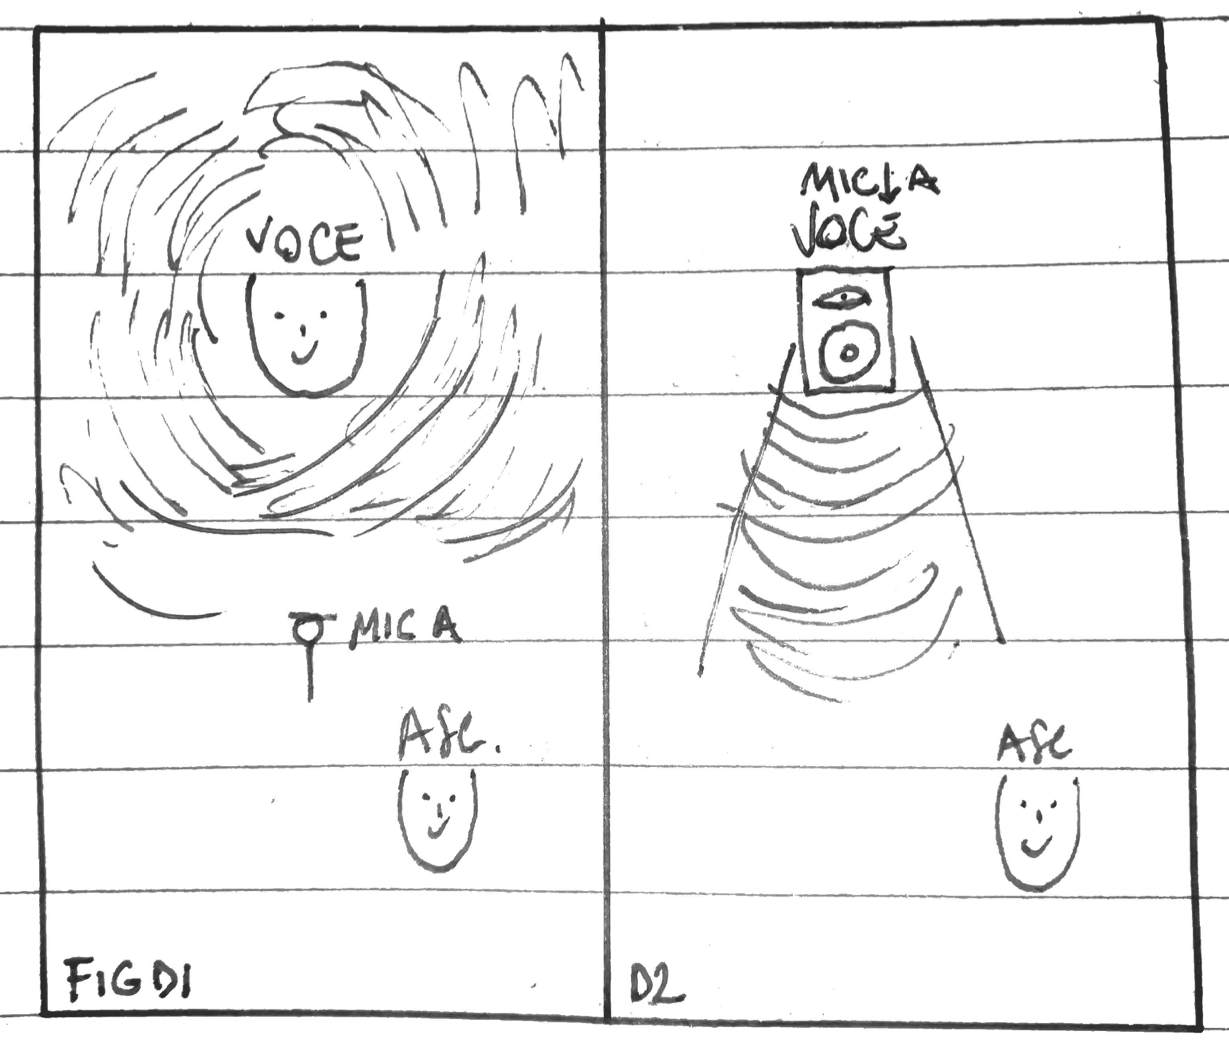
\includegraphics[width=.98\linewidth]{CAPITOLI/1000/IMG/figd1d2.png}
%\caption{}
\label{ee:figd1d2}
\end{center}
\end{figure}


\begin{quote}
When the music is reproduced through a single channel the echoes arrive from the same direction as the direct sound so that confusion result\footnote{Quando la musica viene riprodotta attraverso un singolo canale, gli echi arrivano dalla stessa direzione del suono diretto in modo tale da creare confusione.}.
\end{quote}

Qui si sviluppa tutta la questione, un solo diffusore non è in grado di rappresentare
la solidità originaria, la forma sonora dell'oggetto acustico originario, il suo
rapporto con lo spazio che lo ha modellato. Per comprendere meglio ogni possibile
questione legata alla diffusione sonora, mediante dispositivi elettroacustici ci
vorrebbe un minimo di tempo speso nella sperimentazione con lo strumento altoparlante.
Perché di questo si parla, di uno strumento tecnico, tecnologico, musicale e
profesisonale.

\begin{quote}
Ci sono problemi che alle volte anch'io non capisco, nel senso che se ne porgono
continuamnte di nuovi. È da anni che lavoro e sperimento negli studi di live electronics di
Friburgo, della Sudwestfunk. Si tratta delle trasformazioni in tempo reale del
suono e della voce, e del comporla con lo spazio, usando le tecnologie di oggi,
con i vari altoparlanti disposti nella sala. C'è qualcosa di nuovo solo sul piano
tecnico, perché  se prendiamo la Scuola di S. Marco veneziana di Andrea e Giovanni
Gabrieli, Monteverdi, di Willaert, con le composizioni a più cori, la grande
scuola spagnola all'epoca di Filippo II [\ldots] si faceva musica per otto organi
e quattro cori, cioè si suonava lo spazio come componente musicale, non come poi
la prassi dell'ottocento usa lo spazio, mettendo dentro l'orchestra e quel che
succede succede. Quindi altri studi, anche studi di fisica architettonica, studi
di processi di eco, di riverberazione, di materiali acustici. [\ldots] Qui una
composizione non è  data una volta per sempre, perché per ogni spazio noi dobbiamo
cambiare i programmi dei computer e modificando i rapporti della trasformazione si modifica anche il rapporto acustico; [\ldots] il grande fascino di questo per me
è veramente la non ripetitività. [\ldots] Un interprete non deve studiarsi la
parte ma veramente partecipare. [\ldots] Cioè vedi come noi possiamo con la
tecnologia di oggi studiare molto meglio, cioè studiare in un altro modo. \\
Luigi Nono 1986
\end{quote}

La parabola bacchiana si conclude con una nota autobiografica. Noi, che abbiamo
osservato da vicino la maledizione di Bacco, non possiamo più tacere e seminiamo,
il vento muoverà le orecchie penzolanti e porterà le nostre confessioni altrove.
%%%%%%%%%%%%%%%%%%%%%%%%%%%%%%%%%%%%%%%%%%%%%%%%%%%%%%%%%%%%%%%%%%%%%%%%%%%%%%%%%%%%%%%%%%%%%%%%%% fiune dalle esposizioni

Una singola voce umana, monofonica, sta parlando all'interno di una piccola
stanza, una condizione stereofonica accettabile? In accordo con Blumlein,
Sì! Questo è il primo punto fermo.

Michael Gerzon, dagli anni settanta agli anni novanta, dalle radici dell'era di
Blumlein ha saltato la linea con una dozzina di descrizioni chiare sulla
percezione e tentativi di progettare tecnologie di riproduzione per colmare il
divario rispetto al regno acustico.

\begin{quotation}
The ears and brain localize sounds according to many different mechanism. Among
the most important cues used are low frequency interaural phase (applicable up
to around 2\emph{KHz}, but dominant below 700\emph{Hz}) and localization by
amplitude differences between the two ears, predominantly above about
1\emph{KHz}. While other cues are also important, we have found that satisfying
both these cues, and making them mutually consistent for central listener facing
in any direction, leads to particularly robust and reliable localization
quality.\cite{mg92pdmsss}
\end{quotation}

%%%%%%%%%%%%%%%%%%%%%%%%%%%%%%%%%%%%%%%%%%%%%%%%%%%%%%%%%%%%%%%%%%% SECTION FOUR
%%%%%%%%%%%%%%%%%%%%%%%%%%%%%%%%%%%%%%%%%%%%%%%%%%%%%%%%%%%%%%%%%%%%%%%%%%%%%%%%
\section{Ramificazioni}

Con la profonda conoscenza del significato del tempo tra noi e Blumlein,
possiamo esporre il significato degli altoparlanti meglio di lui. Per l'era
Blumlein, l'altoparlante era lo strumento futuro per un tempo presente migliore.
Il suono riprodotto, alla sua giovane età, era pura magia. Oggi sappiamo bene
quanto siamo insoddisfatti della riproduzione degli altoparlanti. Quando il
primo iPhone è stata l'unica cosa intelligente sul pianeta, è stato fantastico,
un fantastico oggetto di creazione. Oggi con lo stesso oggetto non faremmo
nemmeno una foto. Ascoltare un assolo di violino riprodotto dal miglior
altoparlante sul mercato non è la stessa esperienza della performance reale.
Non è legato alla stereofonia e all'abilità tecnica, è parte integrante del
limite di riproduzione della tecnologia che siamo in grado di realizzare.
%
Sostituendo la voce umana che parla dell'esempio precedente, con un singolo
altoparlante che parla delle registrazioni di quella voce umana perdiamo, come
descritto da Blumlein, la capacità delle orecchie-cervello decifra la relazione
suono-ambiente. Non è più lo stesso ascolto stereofonico. Il numero di fonti è
lo stesso. Entrambi nel loro linguaggio monofonico producono una diversa
condizione di ascolto.%

Nel 1992 Michael Gerzon \cite{mg92pdmsss} disegna una rappresentazione
schematica delle diverse posizioni degli altoparlanti per stereo multispeaker,
da una a cinque:

\begin{quotation}
\ldots we show the loudspeaker layouts considered for frontal stage stereo
using from one (regarding mono as the trivial case of “one-loudspeaker stereo”!)
to five loudspeakers…
\end{quotation}

Esiste una condizione stereo con un solo altoparlante? Davvero si.

Un altoparlante in grado di suonare se stesso, non riproducendo qualcosa di
reale acustico ma producendo un suono che non potrebbe vivere senza un
altoparlante, rappresenta una condizione stereo con caratteristiche generali
simili alla voce parlante. Un rumore rosa filtrato da Butterworth che canta
monofonicamente in una stanza è una condizione di stereofonia.

Per un musicista elettroacustico, gli altoparlanti sono strumenti. La scelta
degli altoparlanti, la conoscenza del loro carattere e delle loro
caratteristiche è un momento necessario per quel musicista. Conoscere il loro
personaggio richiede tempo. Cambiare manualmente la frequenza di un suono
sinusoidale riprodotto da un altoparlante a tre vie, a un metro di distanza,
con le orecchie alla stessa altezza del centro dell'altoparlante, è un buon modo
per dire Ciao! all'altoparlante. Il musicista scoprirà in questo modo che i
suoni prodotti dall'altoparlante cambieranno forma durante lo spazzamento. Forse
vicino al punto di incrocio del crossover troverà alcune peculiarità, altre
strane decorrelazioni di fase ad altissima frequenza. Gli altoparlanti sono
strumenti. Due altoparlanti potrebbero essere il minimo impostato per la
condizione stereofonica di ascolto. Potrebbero essere cantanti elettroacustici
polifonici. Potrebbero anche essere una condizione monofonica, quando non sono
richieste stereofonia o polifonia.%
